\sectiontinyvert{Skeleton} \label{sec:skeleton}

\begin{figure}[tbh]
\centering
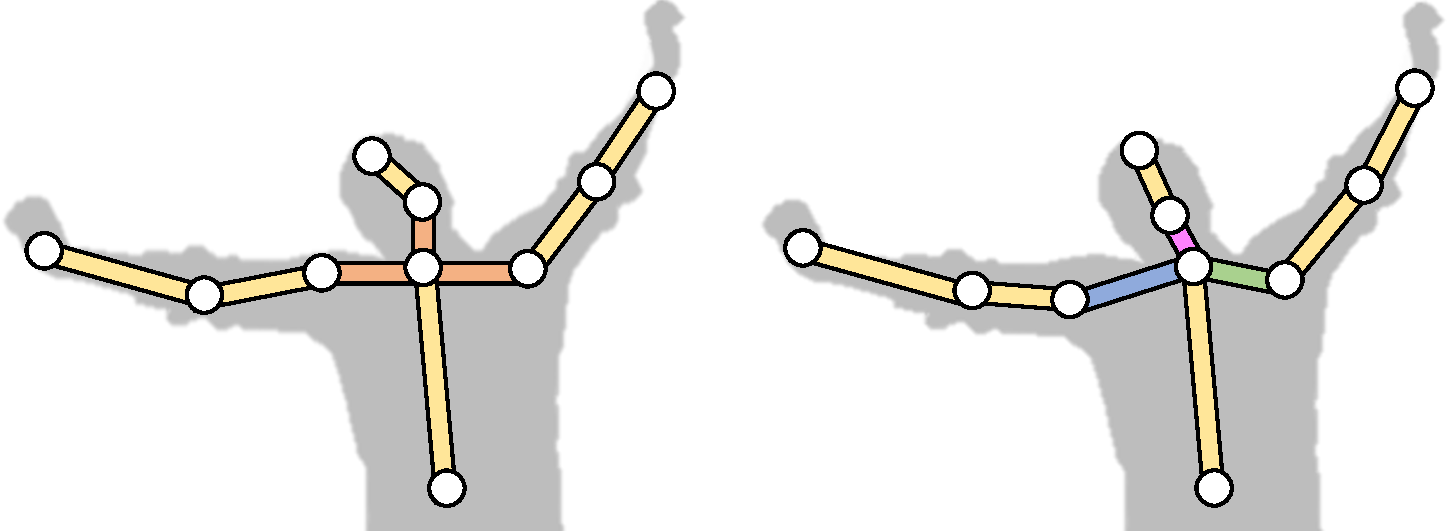
\includegraphics[width=\linewidth]{./images/Skeleton_Difference_Shoulders.pdf}
\setlength{\abovecaptionskip}{-5pt plus 3pt minus 2pt}
\setlength{\belowcaptionskip}{-3pt plus 3pt minus 2pt}
\caption{Skeletal connectivity changes, demonstrated on the neck joint. Left: original connectivity, where shoulders and head are rigidly connected, yielding poor reconstruction. Right: new connectivity, with extra degrees of freedom. }
\label{fig:skeletal_change}
\end{figure}

To better reconstruct the motion in a given video stream, we modify the skeleton connectivity used in our baseline~\cite{shi2020motionet} (\Cref{fig:skeletal_change}).
The root and neck joints of the baseline skeleton are both rigidly attached to the three bones neighboring each of them.
This rigid connectivity constrains the skeleton, e.g., a motion where each shoulder moves forward and the neck moves to the right is impossible.
In order to remove this constraint we add joints that overlap the root and the neck, hence enabling the neighboring bones to move independently of each other. 

The new skeleton connectivity better matches the Human3.6M rotation angles ground-truth, thus, it better matches the way the dataset motions were captured.
The new skeleton improves the mean per joint position error (MPJPE) both in the multi-view setting and the monocular case. The improvements are by  $\sim$4mm and $\sim$6mm for monocular and four cameras setting, respectively.
%\dcc{This last paragraph is need, yes!}


